% !TEX encoding = UTF-8
% !TEX TS-program = pdflatex
% !TEX root = ../tesi.tex

%**************************************************************
\chapter{Processi e metodologie}
\label{cap:processi-metodologie}
%**************************************************************

In questo capitolo verrà fornito una descrizione dei metodi e dei processi messi in atto durante il tirocinio, in particolare riguardo i seguenti argomenti: metodologia agile, programmazione funzionale e il concetto di Dataflow dell'applicazione.

%**************************************************************
\section{Metodologia Agile}
Per lo sviluppo del prodotto è stato deciso di utilizzare una metodologia agile in modo da reagire velocemente a problemi e a cambiamenti così da migliorare ed l'efficienza nella realizzazione della componente. L'azienda ha deciso di utilizzare una metodologia agile simile a SCRUM. Infatti applicare nella sua interezza il metodo SCRUM sarebbe stato impossibile dato il ristretto numero di sviluppatori nel team di sviluppo. \\
Le caratteristiche principali della metodologia agile applicata per la realizzazione di questo progetto sono le seguenti:
\begin{itemize}
	\item \textbf{Modello incrementale}: vengono realizzati rilasci multipli e successivi che aiutano a definire più chiaramente i requisiti più importanti dato che essi verranno implementati per primi. Ogni rilascio corrisponde ad una parte funzionante di applicazione;
	
	\item \textbf{Modello iterativo}: un modello iterativo ha la caratteristica di avere una maggior capacità di adattamento in seguito a problemi di implementazione e cambiamenti nei requisiti da parte del cliente;
	
	\item \textbf{Organizzazione in sprint di sviluppo}: il processo[controlla se è il termine giusto] di codifica viene suddiviso in sprint di sviluppo, data la breve durata del tirocinio curriculare essi avranno una durata di circa 4-5 giorni;
	
	\item \textbf{Backlog}: 
		\begin{itemize}
			\item \textbf{Product Backlog}: rappresenta i requisiti e le funzionalità del prodotto definiti mediante le User Stories;
			\item \textbf{Sprint Backlog}: rappresenta l'insieme delle User Stories da realizzare nello sprint indicato;
		\end{itemize}
	
	\item \textbf{User Stories}: l'idea alla base di uno sviluppo agile è la realizzazione delle User Stories. Ogni user story è definita da una \textbf{descrizione del problema} e da una \textbf{priorità}.
	
	\item \textbf{Riunioni}:
		\begin{itemize}
			\item \textbf{Sprint planning}: per pianificare il lavoro da svolgere durante lo sprint;
			\item \textbf{Sprint review}: riunione retrospettiva per verificare il lavoro svolto durante lo sprint;
			\item \textbf{Backlog refinement}: per aggiungere nuove User Stories o migliorare e/o modificare User Stories già create;
			\item \textbf{Riunioni giornaliere}: per verificare lo svolgimento del lavoro, in questo tirocinio sono state sostituite con comunicazioni telematiche giornaliere.
		\end{itemize}
\end{itemize}
% scrivere descrizione più accurata della metodologie agili applicate
\subsection{Definizione delle User Stories}
Per prima cosa il team di sviluppo si è occupato di realizzare le User Stories. Per definire un singolo elemento è stata utilizzata la seguente struttura:
\begin{longtable} {
		|>{}p{10mm}| 
		|>{}p{70mm}|
		|>{}p{15mm}|
		|>{}p{25mm}|
		>{}p{0mm}}
	\hline
	\textbf{Id} & \textbf{Descrizione} & \textbf{Priorità} & \textbf{Implementato} \\ \hline
	US1.1 & Descrizione dell'user story & A & SI \\ \hline
	\hline
	\caption{Esempio tabella User Story}
\end{longtable}
\noindent
Per ogni descrizione di un user story si possono identificare le seguenti informazioni:
\begin{itemize}
	\item \textbf{Ruolo}: definisce il tipo di utente;
	\item \textbf{Obiettivo}: definisce di che cosa ha bisogno l'utente;
	\item \textbf{Beneficio}: definisce i vantaggi che porta all'utente.
\end{itemize} 
\noindent
La sinteticità e la facilità nel definire le user story porta a vantaggi nella comunicazione tra il team di sviluppo e il cliente, rende più semplice l'aggiornamento dei requisiti e i costi di scrittura e manutenzione delle user stories sono molto bassi.

\subsection{Definizione del Product Backlog}
Uno dei primi obiettivi del progetto posti dal team di sviluppo è stato quello di definire il Product Backlog, cioè i requisiti del prodotto. Per ognuna delle user story precedentemente scritta è stata assegnata una priorità seguendo la seguente legenda:
\begin{longtable} {
		|>{\centering}p{10mm}| 
		|>{}p{25mm}|
		|>{}p{85mm}|
		>{}p{0mm}}
	\hline
	\textbf{A} & \textit{Priorità alta}  & funzionalità necessarie per il corretto funzionamento dell'applicazione \\ \hline
	\textbf{M} & \textit{Priorità media} & funzionalità che migliorano il prodotto \\ \hline
	\textbf{B} & \textit{Priorità bassa} & funzionalità non necessarie per il corretto funzionamento dell'applicazione \\ \hline
	\hline
	\caption{Tabella priorità User Story}
\end{longtable}
\noindent
Questo ci ha permesso di categorizzare le funzionalità principali del componente d'interfaccia grafico da quelle opzionali. Abbiamo quindi popolato il Product Backlog per ordine di \textit{priorità}, in questo modo la suddivisione delle user story per sprint, mediante le riunioni di \textit{Sprint Planning}, è stata chiara e veloce. \\
Infatti abbiamo concentrato le funzionalità principali da implementare nei primi due sprint così da avere già a partire dal terzo sprint una prodotto con le funzionalità principali già implementate.

\section{Programmazione funzionale}

\section{Dataflow dell'applicazione}
Un concetto che è stato discusso molto dal team di sviluppo riguardava il dataflow dell'applicazione. Cioè il modo in cui i dati vengono modificati e utilizzati all'interno del flow dell'applicazione. Durante la prima settimana del tirocinio è stato discusso come verrà gestito lo stato dell'applicazione e in particolare della sua scalabilità. Dato che l'utilizzo di React è un requisito obbligatorio per questo stage abbiamo valutato l'utilizzo del dataflow di React.

\subsection{Dataflow React}
Nella libreria React il dataflow è definito come unidirezionale perchè ogni componente può avere uno stato locale accessibile solo dal componente stesso e può passare informazioni ai suoi componenti figli mediante le \textit{props}. \\
Seguendo questo dataflow però bisognerebbe dare la responsabilità ad un componente grafico di contenere lo stato dell'applicazione nel suo stato locale per poi passare le informazioni mediante le props. Questo rende l'architettura dell'applicazione molto limitata, difficile da manutenere e poco scalabile dato che lo stato di tutta l'applicazione viene gestito da un componente grafico. Come infatti si può vedere nel seguente grafico che rappresenta il dataflow di react abbiamo che il primo componente passa i dati contenuti nel suo state locale ai suoi figli mediante le props che a loro volta passeranno le stesse props ai loro figli.

\begin{minipage}{\linewidth}
	\makebox[\linewidth] {
		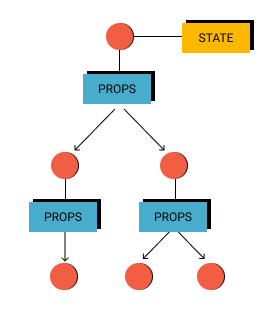
\includegraphics[scale=0.75]{./immagini/dataflow_react.png}
	}
\end{minipage}


\subsection{Redux}
Per garantire garantire scalabilità e facilità di gestione dello stato dell'applicazione abbiamo utilizzato la libreria Redux. Pur essendo un dataflow unidirezionale rende la gestione dello stato dell'applicazione più prevedibile e più manutenibile. Redux si basa su tre principi:
\begin{itemize}
	\item lo stato è l'unica fonte di verità;
	\item lo stato non è modificabile direttamente;
	\item le modifiche avvengono medianti funzioni pure che creano un nuovo stato per evitare side effects.
\end{itemize}
\noindent
Gli elementi dell'architettura di Redux sono i seguenti:
\begin{itemize}
	\item \textbf{Actions}: oggetto che rappresentano il comportamento;
	\item \textbf{Reducers}: funzioni pure che hanno come parametro un Actions e modificano lo stato;
	\item \textbf{Store}: lo Store è un'interfaccia che contiene lo stato dell'applicazione e fornisce funzioni per leggere, modificare e registrare listeners allo stato.
\end{itemize}
\noindent

\subsection{Soluzione}
La soluzione che è stata trovata dal team di sviluppo è stata quella di usare in concomitanza React e Redux. React è stato usato per gestire solo gli aggiornamenti visivi dell'applicazione, mentre Redux per gestire lo stato dell'applicazione. Il dataflow del prodotto è quindi il seguente:
\begin{enumerate}
	\item se lo stato deve cambiare verrà mandata allo Store una richiesta di cambiamento con un Action;
	\item lo Store si occuperà di chiamare un Reducer in modo da modificare lo stato;
	\item lo stato verrà aggiornato e i cambiamenti saranno visibili a tutti i componenti React che sono registrati allo Store.
\end{enumerate}

\noindent
Nella seguente figura è rappresentato il dataflow del componente. \\
In questo modo abbiamo ottenuto un'architettura chiara, manutenibile e abbiamo mantenuto la divisione tra lo stato dell'applicazione e la sua renderizzazione.

\begin{minipage}{\linewidth}
	\makebox[\linewidth] {
		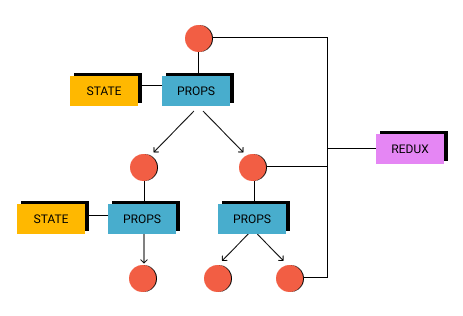
\includegraphics[scale=0.75]{./immagini/dataflow_react_redux.png}
	}
\end{minipage}